\subsection*{Экспериментальная установка}

\textbf{Описание установки}. 1 -- блок питания; 2 -- тумблер включения питания образцов; 3 -- тумблер нагрева нити пирометра; 4 -- кнопка "Нагрев нити"; 5 -- кнопка "охлаждение нити"; 6
-- тумблер переключения образцов; 7 -- регулятор мощности нагрева образцов; 8 -- окуляр пирометра; 9 --
корпус пирометра; 10 -- объектив пирометра; 11 -- переключение диапазонов; 12 -- ручка смещения красного
светофильтра; 13 -- регулировочный винт; 14 -- вольтметр (напряжение на лампе накаливания); 15 -- амперметр (ток через образцы); 16 -- вольтметр в цепи термопары; 17 -- модель АЧТ; 18 трубка с кольцами из
материалов с различной излучательной способностью; 19 -- лампа накаливания; 20 -- неоновая лампочка.

\textbf{Описание образцов}. В работе исследуются:
\begin{itemize}
    \item \textit{Модель абсолютно чёрного тела} -- керамическая трубка, закрытая с одного конца и окружённая для теплоизоляции внешним кожухом. Температура в трубке измеряется с помощью термопары хромель-алюмель.
    \item \textit{Керамическая трубка с набором колец из различных материалов}, нагреваемая изнутри нихромовой спиралью. Материалы колец имеют различную излучательную способность.
    \item \textit{Вольфрамовая нить электрической лампочки}.
\end{itemize}

\begin{figure}[h]
    \centering
    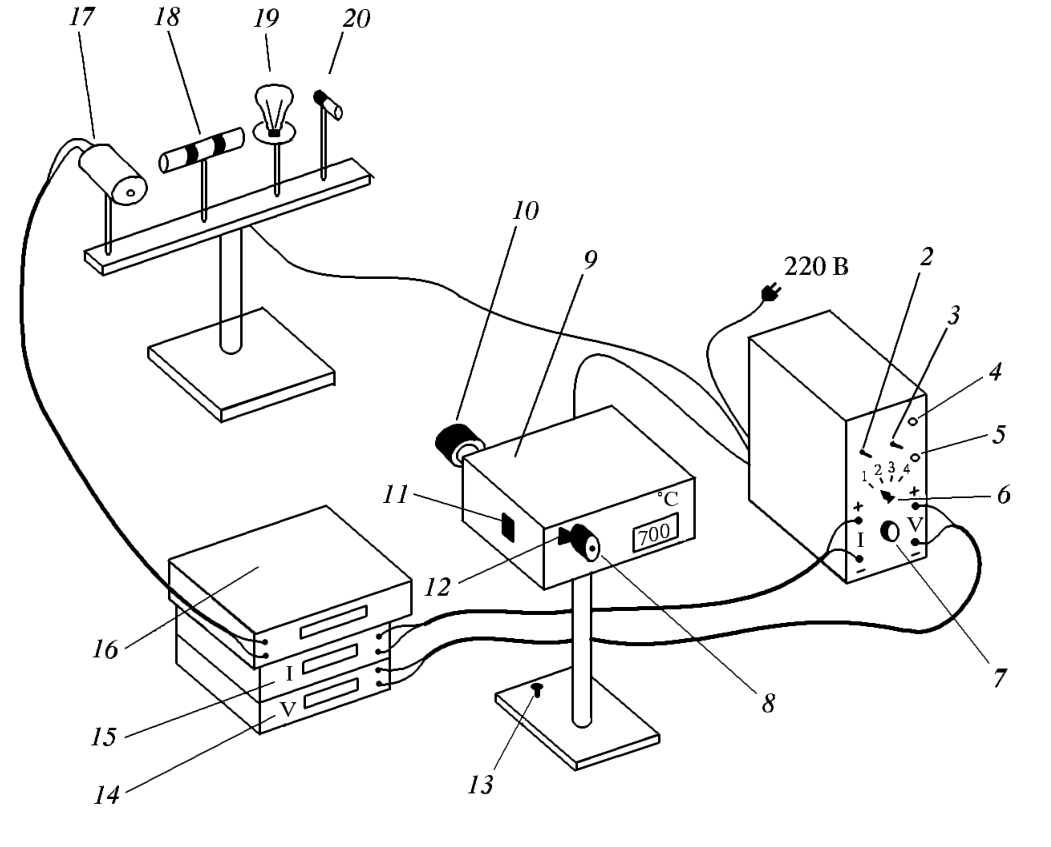
\includegraphics[width=0.6\textwidth]{imgs/exp.png}
    \caption{Схема экспериментальной установки}
    %\label{fig:}
\end{figure}


\newpage


\subsection*{Измерения}

\textbf{Изучение работы пирометра}. Нагрев АЧТ до красного каления (дождавшись стабилизации температуру, судя по показаниям термопары), с помощью пирометра измерим температуру $\sub{t}{pyr}$, сравним её с температурой, полученной по термопаре\footnote{
    Коэффициент перевода: $25.07 \cufrac{$\celc$}{мВ}$.
}  $\sub{t}{therm}$:
\begin{equation*}
    \sub{t}{therm} (45.89 \text{мВ})= 1150 \celc, 
    \hspace{5 mm} 
    \sub{t}{pyr} = [1137, 1140, 1144, 1155] \celc = [0.989, 0.991, 0.995, 1.004] \sub{t}{therm}.
\end{equation*}
Ошибка не превышает $2\%$, так что показанаиям пирометра, по крайней мере для АЧТ в этом диапазоне можно верить. 



\textbf{Изучение яркостной температуры накаленных тел}. Источником нагреваем керамическую трубку с кольцами из различных материалов. Пирометром измерели\footnote{
    Измерения проводлиоись несколько раз, что и обеспечило оценку погрешности каждого из измерений.
}  яркостную температуру поверхности трубки $\sub{t}{surf}$ и каждого из колец $\sub{t}{ring}^{(1)},\, \sub{t}{ring}^{(2)}$:
\begin{equation*}
    \sub{t}{surf} = (850 \pm 10) \celc,
    \hspace{5 mm} 
    \sub{t}{ring}^{(1)} \approx 794 \celc,
    \hspace{5 mm} 
    \sub{t}{ring}^{(2)} \approx 710 \celc.
\end{equation*}
Несовпадение яркостной тепературы обусловлено зависимостью мощности излучения от спектрального коэффициента поглощения, которой, видимо, различен для различных материалов второго образца.



\textbf{Проверка закона Стефана-Больцмана}. Теперь источником нагревается вольфрамовая нить лампы накаливания. С помощью пирометра измерялась яркостная температура нити $\sub{t}{thr}$ (в самом ярком месте). Параллельно снимались значения цифровыми мультиметрами снимались значения тока $I$ и напряжения $U$ на онной. Результаты можно найти в таблице №\ref{tab}.



\begin{table}[ht]
    \caption{Измерение яркостной температуры вольфрамовой нити, как функции мощности}
    \centering
    \begin{tabular}{rrrrrr}
    \toprule
       $U$, В &     $I$, А &    $N$, Вт &   $\Delta N$, Вт &    $t, \celc$ &  $\Delta t, \celc$ \\
    \midrule
    1.65 & 0.481 & 0.79 & 0.02 &  866 &  35 \\
    1.74 & 0.491 & 0.85 & 0.02 &  900 &  37 \\
    2.24 & 0.540 & 1.21 & 0.02 & 1000 &  40 \\
    2.57 & 0.572 & 1.47 & 0.03 & 1100 &  43 \\
    3.31 & 0.638 & 2.11 & 0.04 & 1200 &  46 \\
    3.29 & 0.635 & 2.09 & 0.04 & 1300 &  49 \\
    4.00 & 0.696 & 2.78 & 0.06 & 1400 &  52 \\
    4.74 & 0.754 & 3.57 & 0.07 & 1450 &  53 \\
    4.84 & 0.759 & 3.67 & 0.07 & 1500 &  55 \\
    4.59 & 0.742 & 3.41 & 0.07 & 1500 &  55 \\
    5.32 & 0.798 & 4.25 & 0.08 & 1600 &  58 \\
    6.13 & 0.857 & 5.25 & 0.11 & 1688 &  60 \\
    5.86 & 0.837 & 4.90 & 0.10 & 1700 &  61 \\
    7.00 & 0.915 & 6.40 & 0.13 & 1792 &  63 \\
    7.72 & 0.963 & 7.43 & 0.15 & 1800 &  64 \\
    7.51 & 0.949 & 7.13 & 0.14 & 1833 &  64 \\
    9.22 & 1.053 & 9.71 & 0.19 & 1900 &  67 \\
    \bottomrule
    \end{tabular}
\label{tab}
\end{table}


Погрешность измерения пирометра на основе предыдующих измерений была положена $\sim 3\% \pm 10$, для мультиметров взят $\sim 1\%$ от показаний.


\textbf{Измерение яркостной температуры неоновой лампочки}. Включив неоновую лампочку, пирометром измерим её яркостную температуру $\sub{t}{Ne}$:
\begin{equation*}
    \sub{t}{Ne} = (874 \pm 27) \celc,
\end{equation*}
что, очевидно $\gg 30 \celc$. Ну, так совпало, что переход электронов между энергетическими уровнями неона имеет длину волны схожую, с излучением АЧТ на измеренной температуре. 